\chapter{The periodic table from calculation: configurations, shielding and ionisation}
\sectionmark{The periodic table from calculation}
\label{sec:periodic-trends}
\label{sec:configurations}
\checkedwith{9.5.3-dev}{ce2531fa0}
\index{Periodic trends}
\index{Periodic table|see{Periodic trends}}
\eccexample{Examples > General Chemistry > Atoms}
\helppage{ecce-qm}

The filling order 1s, 2s, 2p, 3s, 3p, 4s, 3d is usually taught as a rule to memorise. Here we read it from calculations instead: the atoms H to Ar, Ca, Cr and Cu, and some of their ions, from the General Chemistry example set. The orbital energies give the configurations and an effective nuclear charge; total energies of atoms and ions give ionisation energies and electron affinities. The rise in ionisation energy across a period, the drop at each alkali metal and the dips at B and O all appear, and so do a few places where the numbers are easy to over-read.
\index{Electron configuration}\index{Configurations|see{Electron configuration}}
\index{Ionisation energy}\index{Ionization energy|see{Ionisation energy}}
\index{Electron affinity}

\section*{This requires}
Nothing beyond ECCE: the calculations are in the General Chemistry example set.

\section{Background}
\index{Aufbau principle}\index{Building-up principle|see{Aufbau principle}}\index{Pauli principle}
\index{Penetration}\index{Shielding}\index{Screening|see{Shielding}}\index{Subshells}
In the orbital picture, the ground state puts the electrons, two per orbital at most, into the orbitals of lowest energy. In hydrogen the energy depends on $n$ alone. In other atoms the electrons screen the nucleus from each other, and an s electron, which penetrates the inner shells, feels more of the nuclear charge than a p electron of the same shell (Chapter~\ref{sec:atomic-orbitals}). The subshells therefore separate, ns below np below nd, and for $n = 3$ and 4 enough that 4s fills before 3d.

\index{Hund's rule}\index{Multiplicity}\index{Spin multiplicity|see{Multiplicity}}
In a partly filled subshell, Hund's first rule puts the electrons in different orbitals with parallel spins. Carbon is then a triplet, nitrogen a quartet, oxygen a triplet again. Note that in a calculation the multiplicity is part of the input: you choose how many electrons are unpaired.

\index{Effective nuclear charge}\index{Zeff@$Z_\mathrm{eff}$|see{Effective nuclear charge}}
The screening can be put into one number, the effective nuclear charge $Z_\mathrm{eff} = Z - S$, where $Z$ is the nuclear charge and $S$ the screening constant. Slater's rules estimate $S$ from the configuration \cite{slater1930}. For an electron in an s or p orbital of shell $n$, every other electron in the same shell contributes 0.35 to $S$ (0.30 within 1s), every electron in shell $n-1$ contributes 0.85, and every electron further in contributes 1.00. For the 2s electron of lithium, $1s^2 2s^1$, the two 1s electrons give $S = 2 \times 0.85 = 1.70$, so that $Z_\mathrm{eff} = 3 - 1.70 = 1.30$. For a 2p electron of neon, $1s^2 2s^2 2p^6$, the seven other $n = 2$ electrons and the two 1s electrons give $S = 7 \times 0.35 + 2 \times 0.85 = 4.15$ and $Z_\mathrm{eff} = 10 - 4.15 = 5.85$.

A second estimate comes from the calculation itself. It treats an orbital of energy $\varepsilon$ as if it were a hydrogen-like orbital of the same $n$, for which $\varepsilon = -Z^2/2n^2$ in hartree, and solves for the charge:
\begin{equation}
	\varepsilon = -\frac{Z_\mathrm{eff}^2}{2n^2}\ \text{hartree}, \qquad
	Z_\mathrm{eff} = n\sqrt{-2\varepsilon/\text{hartree}} .
	\label{eq:zeff}
\end{equation}
The two are not the same thing. An orbital energy contains the repulsion with every other electron, including those of the same shell, and equation~\eqref{eq:zeff} puts all of it into $Z_\mathrm{eff}$.

\index{Koopmans' theorem}\index{Ionisation energy!from orbital energies}\index{Delta SCF@$\Delta$SCF}\index{Relaxation}\index{Electron correlation}\index{HOMO}
The first ionisation energy is $\mathrm{IE} = E(\mathrm{A}^+) - E(\mathrm{A})$, the electron affinity $\mathrm{EA} = E(\mathrm{A}) - E(\mathrm{A}^-)$, positive when the anion is more stable. Both come from two total energies (the $\Delta$SCF route). Koopmans' theorem gives a shortcut for Hartree-Fock: $\mathrm{IE} \approx -\varepsilon_\mathrm{HOMO}$, where HOMO is the highest occupied orbital, if the other orbitals do not change \cite{koopmans1934}. Two errors enter. The remaining electrons relax towards the hole, which makes $-\varepsilon_\mathrm{HOMO}$ too large. Hartree-Fock also leaves out electron correlation, the part of the repulsion between electrons that its average field misses because the electrons in fact avoid each other; the correlation energy is larger in the atom than in the cation and makes the Hartree-Fock IE too small. $\Delta$SCF includes the relaxation but not the correlation. For a density functional such as B3LYP, $-\varepsilon_\mathrm{HOMO}$ is well below the IE.

ECCE gives orbital energies in hartree and the Energy Calculator gives energy differences in kJ/mol, kcal/mol and eV. The conversions used in this chapter are 1~hartree = 27.2114~eV = 2625.50~kJ/mol.

\section{The calculations}
\index{ECCE-QM}\index{Codes!ECCE-QM}\index{Example calculations!General Chemistry}
\index{B3LYP}\index{Basis sets!aug-cc-pVTZ}\index{Basis sets!def2-TZVPD}\index{Basis sets!cc-pVTZ}\index{ROKS}\index{Restricted open shell}
\index{Hartree-Fock}\index{UHF}\index{PBE0}\index{Basis sets!aug-cc-pVDZ}
Three topics of the General Chemistry example set hold the ECCE-QM calculations:
\begin{enumerate}
	\item \menu{Atoms}: the 21 atoms, B3LYP \cite{becke1993}, aug-cc-pVTZ \cite{kendall1992,woon1993} for H to Ar, cc-pVTZ for Ca, def2-TZVPD \cite{rappoport2010} for Cr and Cu. Closed shells are restricted, open shells restricted open-shell (ROKS): the alpha and beta electrons share one set of spatial orbitals. The aug-cc-pVTZ basis is of triple-zeta quality with diffuse functions, which describe the loosely bound outer electrons; cc-pVTZ lacks the diffuse functions, and def2-TZVPD is a triple-zeta basis with diffuse functions from another family.
	\item \menu{Koopmans' theorem}: H to Ar, Hartree-Fock/aug-cc-pVTZ, unrestricted (UHF) for open shells, so that the alpha and beta electrons have orbitals, and orbital energies, of their own.
	\item \menu{Ionisation energies and electron affinities}: Li, Be, C, N, O, F, Ne and their cations (Hartree-Fock/aug-cc-pVTZ); Li, Be, C, N, O, F and their anions (PBE0/aug-cc-pVDZ \cite{adamo1999}).
\end{enumerate}
Each calculation has a note saying what it shows.

\index{MOs panel}\index{Properties list!MOs}\index{MOs panel!Compute}\index{MO Diagram}\index{Properties list!MO Diagram}\index{Orbital energies}
In the Viewer, the \menu{MOs} panel lists the orbitals with their energy and occupation. Select a row and click \ctrl{Compute} to draw the orbital, which tells s from p or d. \menu{Tools > Energy Calculator...} in the Organizer takes two calculations, A then B, and gives \menu{B - A} in kJ/mol, kcal/mol and eV.
\index{Energy Calculator}\index{Tools menu!Energy Calculator...}\index{Energy Calculator!B - A}
\index{Calculating an ionisation energy}\index{Calculating an electron affinity}
\helppage{energy-calculator}

\section{Procedure}
\index{Opening example calculations}\index{File menu!Open Example Calculations}\index{Organizer!Open Example Calculations}\index{Viewer}
\begin{enumerate}
	\item In the Organizer, choose \menu{File > Open Example Calculations}, pick \menu{General Chemistry} and click \menu{OK}.
	\item In \menu{Atoms}, select \menu{Ne}, click \menu{Viewer} and open \menu{MOs}. Read the energies of 1s, 2s and 2p.
	\item Select \menu{Na}, \menu{C}, \menu{N} and \menu{O} in turn. Count the singly occupied orbitals (\menu{Occ \#} 1) and compare with the multiplicity.
	\item Select \menu{Ca}, \menu{Cr} and \menu{Cu}. Find 4s and 3d near the top of the occupied list; \ctrl{Compute} tells which is which.
	\item In \menu{Koopmans' theorem}, open \menu{N\_HF} and \menu{O\_HF} and read the energy of the highest occupied orbital. The \menu{MOs} panel lists the alpha orbitals first and the beta orbitals below them; in an open shell the highest occupied orbital can be a beta one, as in oxygen, so compare the last occupied orbital of each set. Multiply by $-27.2114$ to get the Koopmans IE in eV.
	\index{Koopmans' theorem!in the MOs panel}
	\item In \menu{Koopmans' theorem}, open \menu{Li\_HF}, read \menu{E (Hartree)} of the highest occupied orbital (\menu{Occ \#} 1, the 2s) and calculate $Z_\mathrm{eff} = n\sqrt{-2\varepsilon}$ with $n = 2$ (equation~\eqref{eq:zeff}). Repeat for \menu{Ne\_HF} and \menu{Na\_HF} ($n = 3$), and compare with Slater's rules.
	\index{Effective nuclear charge!calculating}
	\item In \menu{Ionisation energies and electron affinities}, select \menu{N\_HF\_neutral}, Ctrl-click \menu{N\_HF\_cation} and choose \menu{Tools > Energy Calculator...}. \menu{B - A} is the ionisation energy. Repeat for the other pairs.
	\item For an electron affinity, select the anion first (\menu{F\_anion}), then the atom (\menu{F\_PBE0\_neutral}). \menu{B - A} is the electron affinity.
\end{enumerate}

\section{Configurations}
\index{Electron configuration!of the atoms H to Ar}\index{Orbital energies!of the atoms}\index{Penetration!2s and 2p}\index{Neon}\index{Sodium}
Every atom fills its orbitals in the Aufbau order (table~\ref{tab:pt-config}). Neon shows the split of a shell most clearly: 2s at $-1.459$ and 2p at $-0.572$~hartree, 24~eV apart although both have $n = 2$. In sodium the next electron goes into 3s at $-0.125$~hartree, and the 2p has dropped to $-1.156$~hartree, into the core.

\begin{table}[htb]
	\centering\small
	\caption{Atoms H to Ar (B3LYP/aug-cc-pVTZ): multiplicity used, valence configuration and valence orbital energies in hartree. Where singly and doubly occupied p orbitals differ in energy, both are given, singly occupied first.}
	\label{tab:pt-config}
	\begin{tabular}{lcl rr}
		\hline
		Atom & $2S+1$ & Valence configuration & $\varepsilon(n\mathrm{s})$ & $\varepsilon(n\mathrm{p})$ \\
		\hline
		H  & 2 & 1s$^1$         & $-0.319$ & \\
		He & 1 & 1s$^2$         & $-0.658$ & \\
		Li & 2 & 2s$^1$         & $-0.131$ & \\
		Be & 1 & 2s$^2$         & $-0.229$ & \\
		B  & 2 & 2s$^2$2p$^1$   & $-0.371$ & $-0.185$ \\
		C  & 3 & 2s$^2$2p$^2$   & $-0.533$ & $-0.265$ \\
		N  & 4 & 2s$^2$2p$^3$   & $-0.713$ & $-0.355$ \\
		O  & 3 & 2s$^2$2p$^4$   & $-0.942$ & $-0.460$ / $-0.362$ \\
		F  & 2 & 2s$^2$2p$^5$   & $-1.191$ & $-0.565$ / $-0.464$ \\
		Ne & 1 & 2s$^2$2p$^6$   & $-1.459$ & $-0.572$ \\
		Na & 2 & 3s$^1$         & $-0.125$ & \\
		Mg & 1 & 3s$^2$         & $-0.192$ & \\
		Al & 2 & 3s$^2$3p$^1$   & $-0.306$ & $-0.129$ \\
		Si & 3 & 3s$^2$3p$^2$   & $-0.421$ & $-0.191$ \\
		P  & 4 & 3s$^2$3p$^3$   & $-0.540$ & $-0.259$ \\
		S  & 3 & 3s$^2$3p$^4$   & $-0.678$ & $-0.333$ / $-0.274$ \\
		Cl & 2 & 3s$^2$3p$^5$   & $-0.821$ & $-0.407$ / $-0.348$ \\
		Ar & 1 & 3s$^2$3p$^6$   & $-0.968$ & $-0.426$ \\
		\hline
	\end{tabular}
\end{table}

\index{Hund's rule!carbon, nitrogen and oxygen}\index{Carbon}\index{Nitrogen}\index{Oxygen}\index{S2@$S^2$ expectation value}
Carbon has two singly occupied 2p orbitals and the third empty, nitrogen three singly occupied, oxygen one doubly and two singly occupied. These are Hund's arrangements, but be clear with students where they come from: the multiplicity was set in the input. The topic has no singlet carbon or doublet nitrogen, so it does not show that high spin is lower; for that you need a second calculation of the same atom. The expectation value $\langle S^2 \rangle$, under \menu{Properties > Summary > S**2}, confirms the spin state asked for, since $\langle S^2 \rangle = S(S+1)$: 2.000 for the triplets, 3.750 for the quartets, 12.000 for chromium.

\index{Restricted open shell!orbital energies}
Watch out with O, F, S and Cl. In the restricted open-shell calculation the singly occupied 2p orbitals of oxygen lie at $-0.460$~hartree, \emph{below} the doubly occupied one at $-0.362$. This comes from how restricted open-shell orbital energies are defined; it does not mean the unpaired electrons are bound more strongly. The unrestricted Hartree-Fock orbitals show the physics more directly (section~\ref{sec:pt-dips}).

\section{4s and 3d: calcium, chromium and copper}
\index{4s and 3d}\index{3d and 4s|see{4s and 3d}}\index{Calcium}\index{Chromium}\index{Copper}
\index{Chromium!3d5 4s1@3d$^5$4s$^1$}\index{Copper!3d10 4s1@3d$^{10}$4s$^1$}
The \menu{MO Diagram} panel (\menu{Properties > Orbitals > MO Diagram}, with \ctrl{Energies to scale} ticked) gives each level in eV and draws the electrons as arrows; figure~\ref{fig:pt-tm} shows it for copper. In calcium the two outer electrons are in 4s ($-4.11$~eV). Chromium (septet, 3d$^5$4s$^1$) has its 3d at $-4.93$~eV and 4s at $-4.65$~eV; copper (doublet, 3d$^{10}$4s$^1$) has 3d at $-6.90$~eV and 4s at $-5.24$~eV. Across the series 3d falls below 4s, so 4s is the highest occupied orbital and is lost first, which is why Cr$^+$ and Cu$^+$ keep their 3d$^5$ and 3d$^{10}$ cores.

\begin{figure}[htbp]
	\centering
	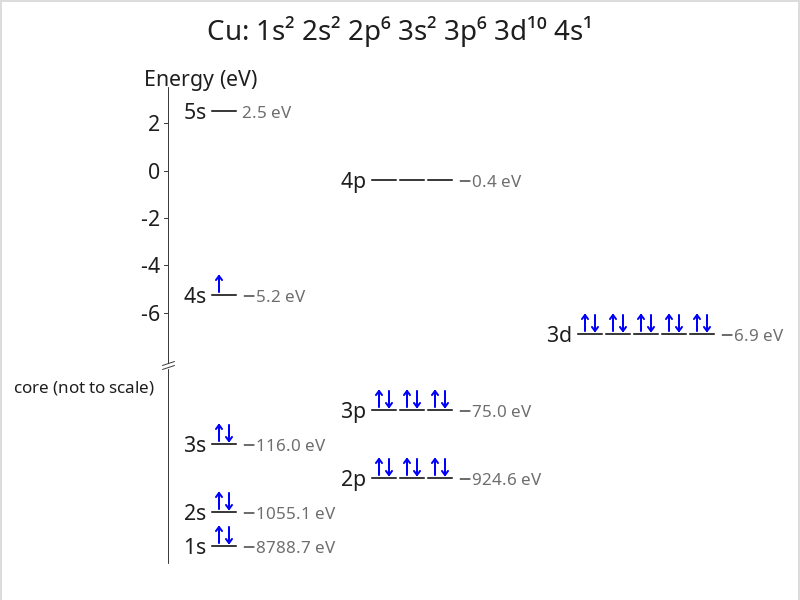
\includegraphics[width=0.8\linewidth]{periodic-trends/tm-mo-cu.ecce-9.5.3-dev.png}
	\caption{The \menu{MO Diagram} panel of copper (B3LYP), energies to scale, with the core below the axis break. The filled 3d level lies below the singly occupied 4s.}
	\label{fig:pt-tm}
\end{figure}

Do not teach the exceptions from this figure. Orbital energies do not decide the configuration; total energies do, and 3d$^4$4s$^2$ chromium or 3d$^9$4s$^2$ copper would each be a separate calculation. The topic has only the observed configurations, so it cannot show that they are the lower ones. The empty orbitals of calcium depend on the basis set, so their order is not to be taught either. \XXX[ check whether ECCE-QM can hold copper in 3d$^9$4s$^2$.]
\index{Exceptions to the Aufbau order}\index{Aufbau principle!exceptions}

\section{Effective nuclear charge}
\index{Effective nuclear charge!from orbital energies}
We take the energy of the highest occupied orbital from the \menu{MOs} panel of the Hartree-Fock calculations in \menu{Koopmans' theorem}, where the column \menu{E (Hartree)} gives it in the unit that equation~\eqref{eq:zeff} needs. For lithium the 2s orbital of \menu{Li\_HF} lies at $-0.1964$~hartree, so that
\begin{equation*}
	Z_\mathrm{eff} = 2\sqrt{2 \times 0.1964} = 2\sqrt{0.3928} = 1.25 ,
\end{equation*}
and for neon the 2p orbitals of \menu{Ne\_HF} lie at $-0.8512$~hartree, which gives $Z_\mathrm{eff} = 2\sqrt{1.7024} = 2.61$. For the third period $n = 3$: the 3s orbital of sodium at $-0.1822$~hartree gives $3\sqrt{0.3644} = 1.81$. Figure~\ref{fig:pt-zeff} shows the same calculation for every atom from H to Ar. Across a period it rises by about 0.3 per element, from 1.25 (Li) to 2.61 (Ne) and from 1.81 (Na) to 3.26 (Ar), because each added proton is only partly screened by the electron added with it. It falls back at each alkali metal, where a new shell starts. The breaks at B, Al, O and S are the same as in the ionisation energies, since this $Z_\mathrm{eff}$ is the Koopmans IE in other units.

\begin{figure}[htbp]
	\centering
	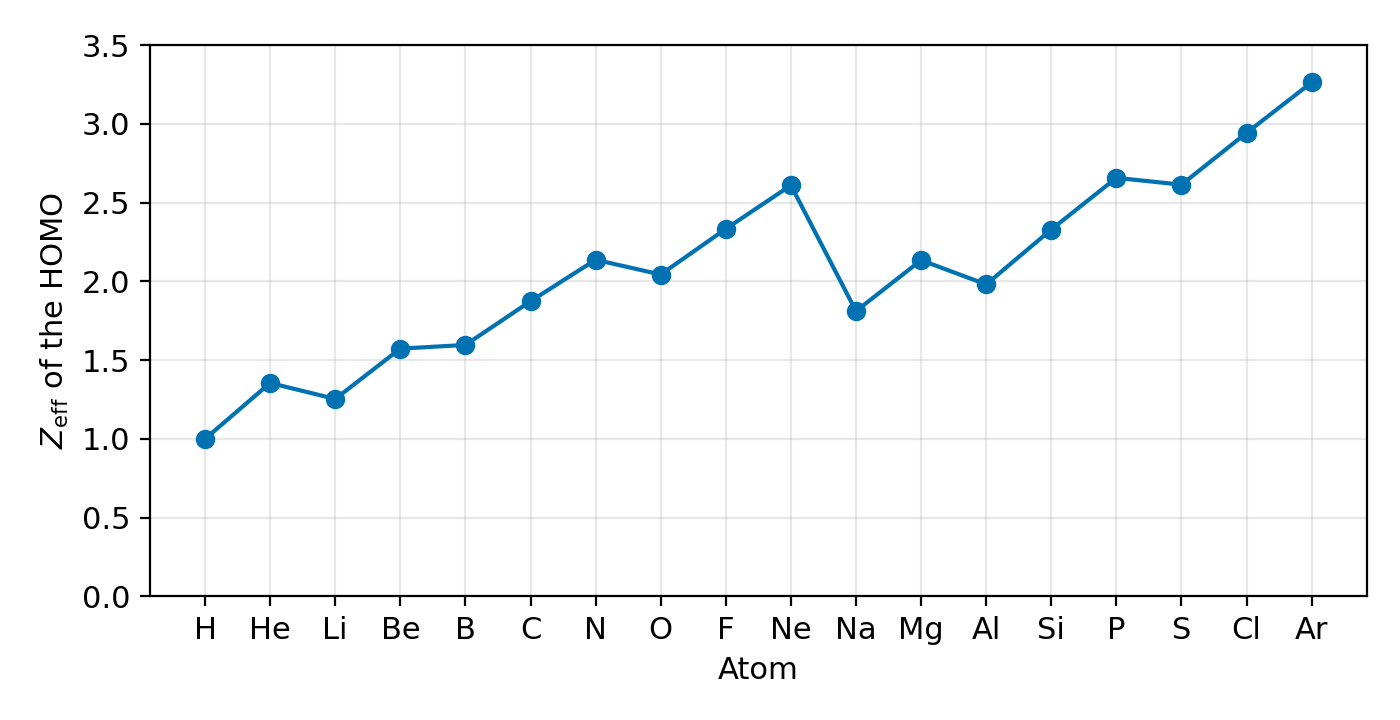
\includegraphics[width=0.85\linewidth]{periodic-trends/zeff.ecce-9.5.2-dev.png}
	\caption{Effective nuclear charge of the highest occupied orbital from equation~\eqref{eq:zeff} and Hartree-Fock/aug-cc-pVTZ orbital energies, plotted from the values in the \menu{MOs} panel.}
	\label{fig:pt-zeff}
\end{figure}

\index{Slater's rules}
For one electron outside a closed shell the estimate agrees with Slater's rules: 1.25 against 1.30 for lithium. For a full shell it does not: Slater gives 5.85 for the 2p of neon, equation~\eqref{eq:zeff} 2.61. The difference is the repulsion with the other seven $n = 2$ electrons, which the orbital energy contains. Teach the trend across a period; the absolute values depend on the definition.

\section{First ionisation energies}
\index{Ionisation energy!across a period}\index{Periodic trends!ionisation energy}\index{Comparing with experiment}
Table~\ref{tab:pt-ie} and figure~\ref{fig:pt-ie} compare the calculated values with experiment \cite{nistasd}. Koopmans' values show the whole textbook curve: the rise across a period, the maxima at the noble gases, the drops to Li and Na, the dips at O, S and Al. Hydrogen gives 13.60~eV, as it must for one electron.

\begin{table}[htb]
	\centering\small
	\caption{First ionisation energies in eV. Koopmans: $-\varepsilon_\mathrm{HOMO}$, Hartree-Fock/aug-cc-pVTZ. $\Delta$SCF: $E(\mathrm{A}^+) - E(\mathrm{A})$, Hartree-Fock/aug-cc-pVTZ. B3LYP: $-\varepsilon_\mathrm{HOMO}$. Experiment: NIST ASD \cite{nistasd}.}
	\label{tab:pt-ie}
	\begin{tabular}{l rrrr}
		\hline
		Atom & Koopmans & $\Delta$SCF & B3LYP & Experiment \\
		\hline
		H  & 13.60 &       &  8.68 & 13.60 \\
		He & 24.98 &       & 17.90 & 24.59 \\
		Li &  5.34 &  5.34 &  3.57 &  5.39 \\
		Be &  8.42 &  8.04 &  6.24 &  9.32 \\
		B  &  8.67 &       &  5.03 &  8.30 \\
		C  & 11.94 & 10.80 &  7.22 & 11.26 \\
		N  & 15.53 & 13.90 &  9.67 & 14.53 \\
		O  & 14.20 & 12.03 &  9.85 & 13.62 \\
		F  & 18.51 & 15.67 & 12.63 & 17.42 \\
		Ne & 23.16 & 19.69 & 15.57 & 21.56 \\
		Na &  4.96 &       &  3.41 &  5.14 \\
		Mg &  6.89 &       &  5.21 &  7.65 \\
		Al &  5.93 &       &  3.51 &  5.99 \\
		Si &  8.20 &       &  5.19 &  8.15 \\
		P  & 10.67 &       &  7.04 & 10.49 \\
		S  & 10.32 &       &  7.46 & 10.36 \\
		Cl & 13.09 &       &  9.47 & 12.97 \\
		Ar & 16.09 &       & 11.59 & 15.76 \\
		\hline
	\end{tabular}
\end{table}

\begin{figure}[htbp]
	\centering
	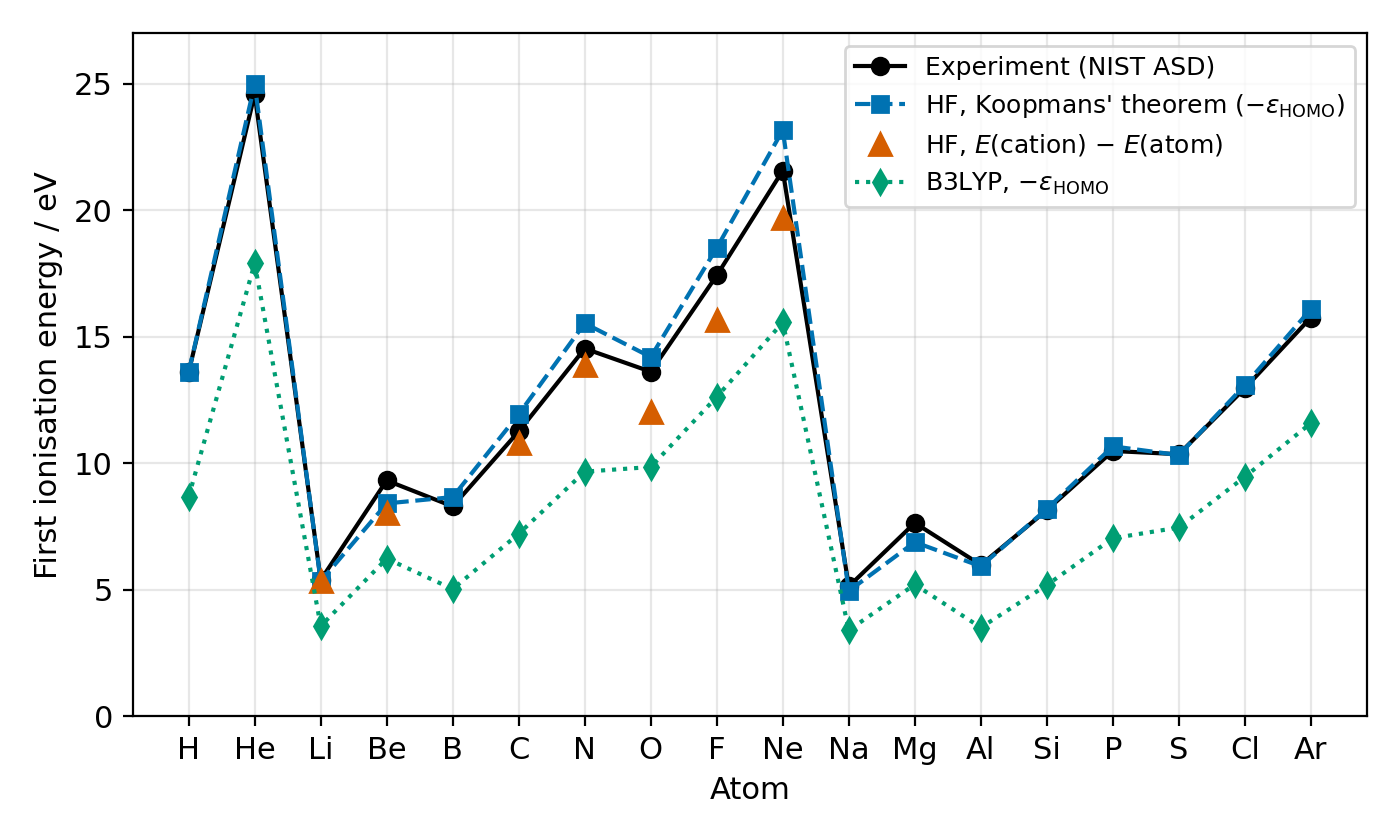
\includegraphics[width=\linewidth]{periodic-trends/ie.ecce-9.5.2-dev.png}
	\caption{First ionisation energies of H to Ar. Black: experiment \cite{nistasd}. Blue: Koopmans. Orange: $\Delta$SCF. Green: $-\varepsilon_\mathrm{HOMO}$ from B3LYP.}
	\label{fig:pt-ie}
\end{figure}

\index{Koopmans' theorem!errors}\index{Relaxation}
$\Delta$SCF is below experiment for all seven atoms, by 0.05~eV at Li and 1.6 to 1.9~eV at O, F and Ne: the missing correlation. Koopmans' values lie above $\Delta$SCF by the relaxation energy (1.1~eV for C, 3.5~eV for Ne). The two errors partly cancel, which is why Koopmans' theorem looks good in figure~\ref{fig:pt-ie}. Do not present it as the more accurate method. For lithium the relaxation is negligible: the Koopmans value, $0.1964~\text{hartree} = 5.344$~eV, and $\Delta$SCF, 5.342~eV from the Energy Calculator, agree to 0.002~eV, because removing the outer electron hardly changes the core.

\index{B3LYP!orbital energies}\index{Density functional theory!HOMO energy}
The B3LYP orbital energies follow the same pattern a few eV lower (8.68~eV for hydrogen). With a density functional, take ionisation energies from total energies, not orbital energies.

\section{The dips at boron and oxygen}
\label{sec:pt-dips}
\index{Ionisation energy!dip at boron}\index{Ionisation energy!dip at oxygen}\index{Boron}\index{Aluminium}\index{Sulfur}
The measured IE falls from Be to B, from N to O, and again from Mg to Al and from P to S. At B and Al the electron removed is the first p electron, which penetrates less than an s electron. At O and S it is the first electron to pair in a p orbital.

\index{Pairing energy}\index{Electron pairing}
The unrestricted Hartree-Fock calculations show the pairing directly. In nitrogen the three alpha 2p orbitals lie at $-0.571$~hartree and there is no beta 2p electron. In oxygen the fourth 2p electron is beta, paired in an orbital with an alpha electron, and lies at $-0.522$~hartree, above all the alpha 2p orbitals. Koopmans gives 14.20~eV for oxygen against 15.53~eV for nitrogen. $\Delta$SCF drops by 1.87~eV, twice the measured 0.92~eV (from the unrounded values 14.534 and 13.618~eV), since Hartree-Fock misses more correlation in oxygen, which has one more electron pair. The cations confirm the counts: O$^+$ is a quartet, N$^+$ a triplet.

\index{Koopmans' theorem!failure for beryllium}\index{Beryllium}
At boron Koopmans' theorem fails: its values \emph{rise} from Be to B (8.42 to 8.67~eV) where experiment falls. Beryllium is 0.90~eV too low, because its 2s$^2$ pair mixes strongly with the nearby empty 2p, a correlation Hartree-Fock omits. Between Mg and Al the gap is wide enough that Koopmans' values fall (6.89 to 5.93~eV). Show the s-to-p dip in the third period.

\section{Electron affinities}
\index{Electron affinity!across a period}\index{Anions}
Table~\ref{tab:pt-ea} gives the electron affinities from PBE0/aug-cc-pVDZ. Fluorine takes up an electron most readily (3.29~eV), filling its 2p. Carbon and oxygen give about 1.4~eV, lithium 0.49~eV. Beryllium and nitrogen come out negative: the anion is higher than the atom. In beryllium the new electron has to go into 2p; in nitrogen it has to pair. These are the same two effects as in the IE dips.

\begin{table}[htb]
	\centering\small
	\caption{Electron affinities, $E(\mathrm{A}) - E(\mathrm{A}^-)$, PBE0/aug-cc-pVDZ, with the multiplicities of atom and anion.}
	\label{tab:pt-ea}
	\begin{tabular}{l cc rr r}
		\hline
		Atom & $2S+1$ atom & $2S+1$ anion & EA / eV & EA / kJ\,mol$^{-1}$ & Experiment / eV \\
		\hline
		Li & 2 & 1 &  0.49 &  47.4 & \XXX \\
		Be & 1 & 2 & $-0.04$ & $-3.8$ & \XXX \\
		C  & 3 & 4 &  1.41 & 136.5 & \XXX \\
		N  & 4 & 3 & $-0.12$ & $-11.7$ & \XXX \\
		O  & 3 & 2 &  1.39 & 134.5 & \XXX \\
		F  & 2 & 1 &  3.29 & 317.6 & \XXX \\
		\hline
	\end{tabular}
\end{table}

\index{Electron affinity!negative}
A negative EA in a finite basis set is only an indication: an unbound anion has no stable state, and its computed energy depends on the basis set. Teach the sign, not the size. Never read an EA from the anion's orbital energies: the HOMO of Li$^-$ and C$^-$ lies above zero, although both anions are bound by total energy.

\section{History}
\index{History!Koopmans}\index{History!Slater}\index{History!Hund}
Slater published his screening rules in 1930 \cite{slater1930}, Koopmans his theorem in 1934 \cite{koopmans1934}. Hund's rules came from his analysis of atomic spectra \XXX[ citation and year].
